\documentclass[12pt, a4paper]{article}

\usepackage{amsmath, amssymb, amsthm}
\usepackage{geometry}
\usepackage{booktabs}
\usepackage{array}
\usepackage{hyperref}
\usepackage{xcolor}
\usepackage{tcolorbox}
\usepackage{enumitem}
\usepackage{parskip}
\usepackage{tikz}
\usetikzlibrary{arrows.meta, positioning, calc}

\geometry{margin=2.5cm}

\newif\ifstudentmode
\studentmodefalse
\ifx\studentflag\undefined\else\studentmodetrue\fi

\newcommand{\sol}[2][6cm]{%
  \ifstudentmode\underline{\hspace{#1}}\else{#2}\fi}
\newcommand{\soleq}[2][3cm]{%
  \ifstudentmode
    \par\vspace{4pt}\noindent\rule{\linewidth}{0.5pt}\\[#1]%
    \noindent\rule{\linewidth}{0.5pt}\par\vspace{4pt}%
  \else\[#2\]\fi}

\definecolor{mainblue}{RGB}{30, 100, 180}
\definecolor{boxbg}{RGB}{235, 243, 255}
\definecolor{notebg}{RGB}{255, 248, 230}
\definecolor{warnbg}{RGB}{255, 235, 235}
\definecolor{greenbg}{RGB}{230, 255, 235}

\tcbuselibrary{skins, breakable}

\newtcolorbox{resultbox}{colback=boxbg,colframe=mainblue,boxrule=1.2pt,arc=4pt,
  title={Result},fonttitle=\bfseries\color{white},coltitle=white,
  attach boxed title to top left={yshift=-2mm,xshift=4mm},
  boxed title style={colback=mainblue,arc=3pt}}

\newtcolorbox{notebox}{colback=notebg,colframe=orange!70!black,
  boxrule=1pt,arc=4pt,left=4pt,right=4pt}

\newtcolorbox{warnbox}{colback=warnbg,colframe=red!60!black,
  boxrule=1pt,arc=4pt,left=4pt,right=4pt}

\newtcolorbox{stepbox}[1]{colback=greenbg,colframe=green!50!black,
  boxrule=1pt,arc=4pt,title={#1},fonttitle=\bfseries,coltitle=green!30!black}

\theoremstyle{definition}
\newtheorem{example}{Example}[section]

\newcommand{\yhat}{\hat{y}}
\newcommand{\sigmoid}{\sigma}

\begin{document}

\begin{center}
  {\LARGE \textbf{Section 4.2: Dropout}} \\[0.3em]
  {\large\itshape Regularising by Randomly Silencing Neurons} \\[0.5em]
  {\large AI Class --- Lecture Notes}%
  \ifstudentmode\quad{\normalsize\color{gray}[Student Copy]}\fi
\end{center}

\vspace{1em}\hrule\vspace{1.5em}

% ══════════════════════════════════════════════════════════════════════════════
\section{The Idea}

L1/L2 regularisation discourages large weights.
\textbf{Dropout} takes a different approach: during each training step,
randomly \emph{silence} a fraction of neurons --- set their output to zero.

\begin{center}
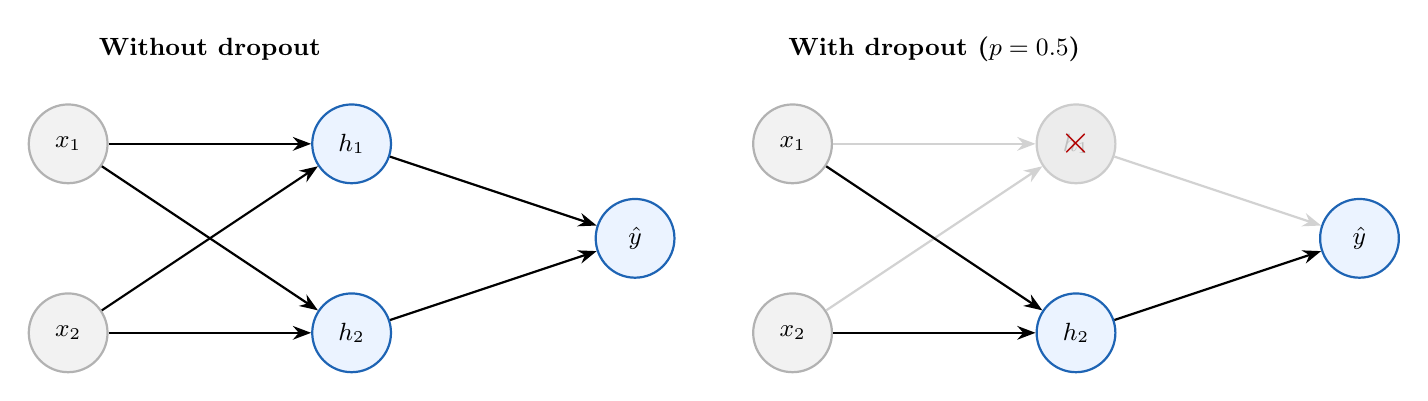
\begin{tikzpicture}[
  neuron/.style={circle,draw=mainblue,fill=boxbg,minimum size=1.0cm,thick,font=\small},
  dead/.style={circle,draw=gray!40,fill=gray!15,minimum size=1.0cm,thick,font=\small,
               text=gray!50},
  input/.style={circle,draw=gray!60,fill=gray!10,minimum size=1.0cm,thick,font=\small},
  >=Stealth
]
  % Normal network
  \node[font=\small\bfseries] at (1.8, 2.4) {Without dropout};
  \node[input]  (x1a) at (0,  1.2) {$x_1$};
  \node[input]  (x2a) at (0, -1.2) {$x_2$};
  \node[neuron] (h1a) at (3.6,  1.2) {$h_1$};
  \node[neuron] (h2a) at (3.6, -1.2) {$h_2$};
  \node[neuron] (ya)  at (7.2,  0)   {$\yhat$};
  \foreach \s in {x1a,x2a} \foreach \t in {h1a,h2a}
    \draw[->,thick] (\s) -- (\t);
  \foreach \s in {h1a,h2a}
    \draw[->,thick] (\s) -- (ya);

  % Dropout network
  \node[font=\small\bfseries] at (11.0, 2.4) {With dropout ($p=0.5$)};
  \node[input]  (x1b) at (9.2,  1.2) {$x_1$};
  \node[input]  (x2b) at (9.2, -1.2) {$x_2$};
  \node[dead]   (h1b) at (12.8,  1.2) {$h_1$};   % dropped
  \node[neuron] (h2b) at (12.8, -1.2) {$h_2$};
  \node[neuron] (yb)  at (16.4,  0)   {$\yhat$};
  \draw[->,thick,gray!35] (x1b) -- (h1b);
  \draw[->,thick,gray!35] (x2b) -- (h1b);
  \draw[->,thick] (x1b) -- (h2b);
  \draw[->,thick] (x2b) -- (h2b);
  \draw[->,thick,gray!35] (h1b) -- (yb);
  \draw[->,thick] (h2b) -- (yb);
  % X mark on h1b
  \node[red!70!black, font=\Large\bfseries] at (12.8, 1.2) {$\times$};
\end{tikzpicture}
\end{center}

Each training step uses a \emph{different} random mask.
The network can never rely on any single neuron being present, so it is
forced to learn \textbf{redundant, robust representations}.

% ══════════════════════════════════════════════════════════════════════════════
\section{The Mechanism: Inverted Dropout}

Let $p$ be the \textbf{dropout probability} (fraction of neurons silenced).

For each neuron, independently:
\begin{enumerate}[nosep]
  \item Draw a Bernoulli sample: keep with probability $(1-p)$, drop with
        probability $p$.
  \item If dropped: set the neuron's output to $0$.
  \item If kept: \textbf{scale up} by $\dfrac{1}{1-p}$.
\end{enumerate}

\begin{resultbox}
\textbf{Why scale up?}
Without scaling, the expected output of a kept neuron is $(1-p)\,h$
(it is alive with probability $1-p$, dead otherwise).
Multiplying by $\dfrac{1}{1-p}$ restores the expected value to $h$,
so the output layer sees the same expected input whether or not dropout
is active.  At \textbf{inference time}, dropout is turned off entirely
and no scaling is applied.
\end{resultbox}

% ══════════════════════════════════════════════════════════════════════════════
\section{Hand-Calculated Example}

We use the XOR network from Section 3.3.  After the hidden layer we have:
\[
  h_1 = 0.500, \qquad h_2 = 0.622, \qquad p = 0.5.
\]

\subsection{Case A: $h_1$ is dropped, $h_2$ is kept}

\begin{stepbox}{Apply mask and scale}
\[
  h_1^{\text{eff}} = 0 \qquad (\text{dropped})
\]
\[
  h_2^{\text{eff}} = \frac{h_2}{1-p} = \frac{0.622}{0.5} = \sol[3cm]{1.244}
\]
\end{stepbox}

\begin{stepbox}{Forward pass to output}
\[
  z^{(2)} = 0.5\,(0) + 0.5\,(1.244) + 0 = \sol[3cm]{0.622}
\]
\[
  \yhat = \sigmoid(0.622) \approx \sol[3cm]{0.651}
\]
\end{stepbox}

\subsection{Case B: $h_1$ is kept, $h_2$ is dropped}

\begin{stepbox}{Apply mask and scale}
\[
  h_1^{\text{eff}} = \frac{0.500}{0.5} = \sol[3cm]{1.000}
  \qquad
  h_2^{\text{eff}} = 0 \qquad (\text{dropped})
\]
\end{stepbox}

\begin{stepbox}{Forward pass to output}
\[
  z^{(2)} = 0.5\,(1.000) + 0.5\,(0) + 0 = \sol[3cm]{0.500}
\]
\[
  \yhat = \sigmoid(0.500) = \sol[3cm]{0.622}
\]
\end{stepbox}

\subsection{Summary: three possible forward passes}

\begin{center}
\renewcommand{\arraystretch}{1.4}
\begin{tabular}{lccc}
\toprule
Scenario & $h_1^{\text{eff}}$ & $h_2^{\text{eff}}$ & $\yhat$ \\
\midrule
No dropout (inference) & $0.500$ & $0.622$ & $0.637$ \\
Case A: $h_1$ dropped  & $0$     & $1.244$ & $0.651$ \\
Case B: $h_2$ dropped  & $1.000$ & $0$     & $0.622$ \\
\bottomrule
\end{tabular}
\end{center}

Each training step sees a different network, producing a different
prediction and different gradients.
Over many steps, the weights must learn to work in \emph{any} subset ---
which forces robustness.

% ══════════════════════════════════════════════════════════════════════════════
\section{Training vs Inference}

\begin{center}
\renewcommand{\arraystretch}{1.3}
\begin{tabular}{lll}
\toprule
Phase & Dropout active? & Scaling? \\
\midrule
Training   & Yes — random mask each step & Scale kept neurons by $\frac{1}{1-p}$ \\
Inference  & No — all neurons active      & No scaling needed \\
\bottomrule
\end{tabular}
\end{center}

\begin{warnbox}
\textbf{Common mistake:} forgetting to call \texttt{model.eval()} before
evaluating on the test set.  In eval mode PyTorch automatically disables
dropout; in training mode it is active.  Always switch modes explicitly.
\end{warnbox}

% ══════════════════════════════════════════════════════════════════════════════
\section{Choosing the Dropout Rate $p$}

\begin{center}
\renewcommand{\arraystretch}{1.3}
\begin{tabular}{lll}
\toprule
$p$ & Typical use & Note \\
\midrule
$0.2$--$0.3$ & Mild regularisation, small networks & Safe default to start \\
$0.5$        & Standard, fully-connected layers    & Most cited in literature \\
$0.7$        & Aggressive, large networks          & Risk of underfitting \\
\bottomrule
\end{tabular}
\end{center}

\begin{notebox}
Dropout is usually \emph{not} applied to the output layer, and in
convolutional networks it is typically placed only after the
fully-connected layers.  See \texttt{code\_examples.py} for placement.
\end{notebox}

\end{document}
